\chapterimage{header.jpg} 
\chapter{Introduction}
\bigskip

\noindent This guide provides a brief introduction to the models that make up the Coupled Ocean-Atmosphere-Wave-Sediment Transport Modeling System
(COAWST), as well as the additional user settings required for specific projects. As shown in Figure \textcolor{bleu_cite} {\ref{coawstestruct}},
COAWST uses several models and programs that will be presented below:


\bigskip

\begin{itemize}
    \item \textbf{COAWST}: Core of the coupled numerical modeling system. More information in the section \textcolor{bleu_cite}{\ref{coawstsecao}};
    \item \textbf{ROMS}: The hydrodynamic model. More information in the Section \textcolor {bleu_cite}{\ref{romssecao}};
    \item \textbf{Sea Ice}: The sea ice model, coupled to ROMS. In this guide we use the Budgell's Sea Ice Model. More information in the Section \textcolor{bleu_cite}{\ref{seaicesecao}};
    \item \textbf{WRF}: The atmospheric model. More information in the Section \textcolor{bleu_cite}{\ref{secaowrf}};
    \item \textit{\textbf{wrf}}: Executable program to start the WRF atmospheric simulation. More information in the section \textcolor{bleu_cite}{\ref{wrfsecao2}};
    \item \textit{\textbf{real}}: Executable program to generate the initial condition and the boundary forces of the WRF. More information in the Section \textcolor{bleu_cite}{\ref{realsecao}};
    \item \textit{\textbf{WPS}}: Package with three programs to generate the files to be used in \textit {real}. More information in the Section \textcolor{bleu_cite}{\ref{wpssecao}};
    \item \textit{\textbf{geogrid}}: Program to, mainly, generate the WRF grid domain. More information in the section \textcolor{bleu_cite}{\ref{geowps}};
    \item \textit{\textbf{ungrib}}: Briefly, the program that extracts the data in \textit{GRIB} format. More information in the Section \textcolor{bleu_cite}{\ref{ungribsecao}};   
    \item \textit{\textbf{metgrid}}: Briefly, the program that interpolates the data generated by \textit {ungrib}. More information in the Section \textcolor{bleu_cite}{\ref {metgridsecao}};    
    \item \textbf{SWAN}: The wave model. More information in the Section \textcolor{bleu_cite}{\ref{swansecao}};
    \item \textbf{MCT}: The set of codes that couples the previous models. More information in the Section \textcolor{bleu_cite}{\ref{mctsecao}};
    \item \textbf{SCRIP}: Package that interpolates and remaps the model's grids to allow the models to be coupled. More information in the section \textcolor{bleu_cite}{\ref{scripsecao}}.
\end{itemize}   
\bigskip

\begin{figure} 
    \footnotesize
    \centering
    \begin{forest}
        for tree={font=\sffamily, %grow'=0,
        folder indent=1.1em, folder icons,
        edge=solid}
        [COAWST 
        [SWAN]
        [Lib
            [SCRIP]
            [MCT]]
        [ROMS
        [Sea Ice]]
        [WRF
            [WPS
                [\textit{ungrib}]
                [\textit{geogrid}]               
                [\textit{metgrid}]]
                [\textit{real}, is file]  
                [\textit{wrf}, is file]
        ]
        ]
      \end{forest}
  \caption{COAWST folder structure.}\label{coawstestruct}
\end{figure}
\bigskip
\pagebreak

\noindent When writing this guide, we chosed to use Python as a programming language for some steps. It is a programming language designed with a philosophy of emphasizing the 
importance of the programmer's effort over the computational effort and prioritizes code readability over speed or expressiveness. The language has a wide and active community,
which facilitates the search information by the user, as there is an extensive collection of libraries and documents on the internet.
\bigskip

\noindent Python (\textcolor{bleu_cite}{\href{http://python.org}{\textit{http://python.org}}}) offers great help for beginners, providing introductions about the 
language and also a guide to use Python for scienfic purposes. 
\bigskip

\noindent We also use MATLAB as a language. It is a paid, but high-performance interactive software focused on the numerical calculation. The MATLAB Answers website is a platform created 
to offer help to the users about the language. The site is avaliable at
\textit{\textcolor{bleu_cite}{\href{https://www.mathworks.com/matlabcentral/answers/index}{https://www.mathworks.com/matlabcentral/answers/index}}}.




%%%%%%%%%%%%%%%%%% ROMS %%%%%%%%%%%%%%%%%%%%

\section{Regional Ocean Modeling System}\index{Regional Ocean Modeling System}\label{romssecao}
\bigskip
\noindent The Regional Ocean Modeling System (ROMS; \cite{Shchepetkin2005}) is a three-dimensional ocean model with free surface, vertical sigma coordinate 
with sigma vertical coordinates (that follow the terrain) and solve primitive equations. The model uses the Reynolds average and the finite difference method to 
solve the Navier-Stokes equations using hydrostatic and Boussinesq approximations (\cite{Haidvogel2008}).
\bigskip

\noindent The hydrostatic equations of momentum use a split-explicit time-step scheme, where the barotropic and baroclinic modes are solved separately, in
different finite numbers of steps of time, to solve the free surface equations and it is integrated vertically. This structure separate time-steps frames maintains 
the volume conservation and consistency preservation that are necessary for the tracers (\cite{Shchepetkin2005, Haidvogel2008}).
\bigskip

\noindent The model solves the horizontally equations through orthogonal curvilinear coordinates of the Arakawa-C grid type (\cite{Arakawa1977}). Vertically, the 
coordinates follow the features of the terrain and allow you to adjust the resolution along the water column. To guarantee the conservation of momentum, the grid uses
econd order finite differences (\cite{Haidvogel2008}).
\bigskip

\noindent ROMS is a model that has free code and its development has the contribution of the user community. Currently, the version used in COAWST is managed by Dr.
Hernan Arango of Rutgers University. To access the model code, is necessary to register on the ROMS website (\textcolor{bleu_cite}{\href{https://www.myroms.org/}{\textit{https://www.myroms.org/}}})
The site has a extremely useful and very active forum to discuss about questions and suggestions. You can access here:
\textcolor{bleu_cite}{\href{https://www.myroms.org/forum}{\textit{https://www.myroms.org/forum}}}.
\bigskip

\noindent We recommend to read the ROMS Technical Manual, written by \textcite{hedstrom2018}. This manual has several
information about the equations and algorithms of the model and examples of test cases.

%%%%%%%%%%%%%%%%%%%% Sea Ice %%%%%%%%%%%%%%%%%%%%

\section{Budgell's Sea Ice Model}\index{Budgell's Sea Ice Model}\label{seaicesecao}
\bigskip

\noindent The Sea Ice Model, proposed by \textcite{Budgell2005}, has the same time and grid steps as the ROMS model and shares the same parallel encoding structure for use with Message Passing Import (MPI). 
Thus, allows dynamic and thermodynamic modeling where sea ice predominates, such as at high latitudes.
\bigskip

\noindent The main attributes of the model, according to \textcite{hedstrom2018}, are:
\bigskip
\begin{itemize}
    \item \textcite{Hunke1997} and \textcite{Hunke2001} elasctic-viscous-plastic dynamics;
    \item \textcite{Mellor1989} thermodynamics;
    \item Orthogonal-curvilinear coordinates;
    \item \textcite{Arakawa1977} grid;
    \item \textcite{Smolarkiewicz1990} advection of tracers;
    \item \textcite{Lemieux2015} landfast ice parameterization.
\end{itemize}
\bigskip


%%%%%%%%%%%%%%%%%%%% WRF %%%%%%%%%%%%%%%%%%%%

\section{Weather Research \& Forecasting Model}\index{Weather Research \& Forecasting Model}\label{secaowrf}
\bigskip

\noindent The Weather Research and Forecasting (WRF; \cite{Skamarock2008}) is a model developed by the National Centers for nvironmental Prediction (NCEP), the National Center for 
Atmospheric Research (NCAR) and research groups from different universities.
\bigskip

\noindent To integrate the governing equations over time, the Advanced Research WRF (ARW) uses low frequency modes that are integrated using the third-order Runge-Kutta scheme, 
and the integrated acoustic and gravity (high frequency) modes with a lower time step. By this way, the numerical stability is maintained through a “forward-backward” scheme for
acoustic modes that propagate horizontally and an implicit scheme for acoustic modes for vertical propagation and buoyancy oscillations (\cite{Skamarock2008}).
\bigskip

\noindent The WRF model uses an Arakawa-C type grid (\cite{Arakawa1977}), where normal speeds are staggered halfway through the grid of thermodynamic variables, as shown in the 
schematic representation illustrated in Figure \textcolor{bleu_cite}{\ref{gradeswrf}}.
\bigskip

\begin{figure}[H]
    \centering
    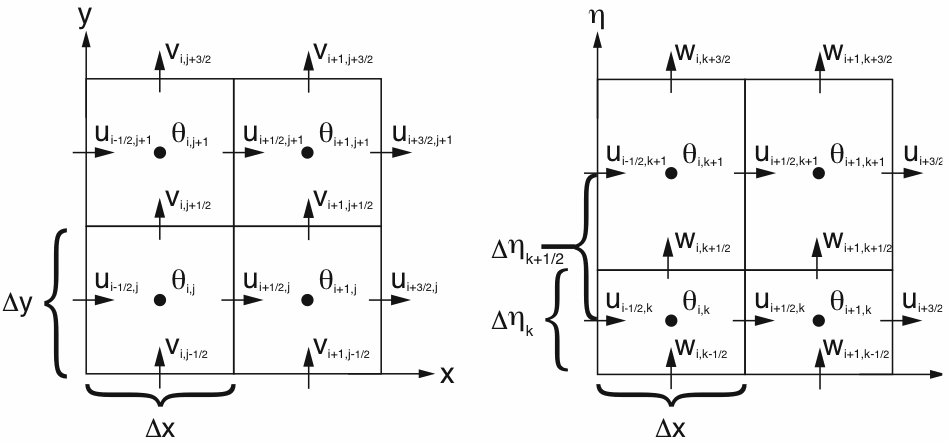
\includegraphics[width=0.75\textwidth]{grid_new.png}
    \caption{Horizontal and vertical grid of Weather Research and Forecast (WRF) using the Arawaka-C grid. The horizontal and vertical components
                        of velocity (\textbf{u}, \textbf{v} and \textbf{w}) are positioned along the faces of the grids and the thermodynamic variables
                        (\straighttheta) are positioned in the center of each grid. \newline Author: \textcite{Skamarock2008}.}
    \label{gradeswrf}
\end{figure}
\bigskip

\noindent It is important to note that the WRF, without coupling with other models, simulates the surface roughness based on the ratio of roughness to wind 
shear proposed by \textcite{Charnock1955}, as exemplified in the following equation \textcolor{bleu_cite}{\ref{equacao1}}:
\bigskip

\begin{equation}
Z_{0} = Z_{ch} \frac{u_{*}^{2}}{g}
\label{equacao1}
\end{equation}

\bigskip

\noindent Where \textit{Z\textsubscript{0}} é a roughness, \textit{Z\textsubscript{ch}} is the Charnock parameter (a dimensionless value of 0,018), \textit{u\textsubscript{*}} 
the frictional speed (m/s) and \textit{g} the gravity acceleration(9,81 m/s\textsuperscript{2}).
\bigskip

\noindent The WRF is avaliable at: \textcolor{bleu_cite}{\href{http://www2.mmm.ucar.edu/wrf/users/download/get\_source.html}{\textit{http://www2.mmm.ucar.edu/wrf/users/download/get\_source.html}}}.
\bigskip

%%%%%%%%%%%%%%%%%%% SWAN %%%%%%%%%%%%%%%%

\section{Simulating Waves Nearshore}\index{Simulating Waves Nearshore}\label{swansecao}
\bigskip

\noindent The Simulating Waves Nearshore (SWAN; \cite{Booij1999, Booij1996}) is a third generation model,
designed to simulate coastal regions with shallow waters and local currents. The model is widely used in the numerical forecast of the Simulating Waves Nearshore (SWAN; \cite{Booij1999, Booij1996}) is a third generation model,
designed to compute in coastal regions with shallow waters and local currents. The model is widely used in the numerical forecast of waves in coastal regions, estuaries,  channels and 
others, being able to use fields of wind, bathymetry and currents provided by other models \parencite{Booij1999, Booij1996}.
\bigskip

\noindent \textcite{Dasilva2013} and \textcite{Booij1999,Booij1996} list the main characteristics of the SWAN:
\bigskip

\begin{itemize}
\item Wave propagation in time and space, shoaling, refraction due to current and depth, frequency shifting due to currents and non-stationary depth;
\item Wave generation by wind;
\item Whitecapping, bottom friction and depth-induced breaking;
\item Dissipation due to aquatic vegetation, turbulent flow and viscous fluid mud;
\item Wave-induced set-up;
\item Propagation from laboratory up to global scales;
\item Transmission through and reflection (specular and diffuse) against obstacles;
\item Diffraction.
\end{itemize}
\bigskip

More features can be found in SWAN website, avaliable at: \textcolor{bleu_cite}{\href{http://swanmodel.sourceforge.net/}{\textit{http://swanmodel.sourceforge.net/}}}.

%%%%%%%%%%%%%%%%%%% MCT %%%%%%%%%%%%%%%%
\section{Model Coupling Toolkit}\index{Model Coupling Toolkit}\label{mctsecao}
\bigskip

\noindent  The Model Coupling Toolkip (MCT; \cite{Larson2005, Jacob2005, Warner2008}) is a set of open-source scripts, written in Fortran90 that allow the transmission 
and transformation of the different data necessary for model coupling. During initialization, model domains are broken down into segments that are distributed
between processors, allowing models to be coupled also in parallel.
\bigskip

\noindent According to the MCT website, (\textcolor{bleu_cite}{\href{http://www.mcs.anl.gov/research/projects/mct/}{\textit{http://www.mcs.anl.gov/research/projects/mct/}}}), 
the toolkit provides the following core coupling services:
\bigskip

\begin{itemize}
\item A component model registry;
\item Domain decomposition descriptors;
\item A time averaging and accumulation buffer datatype;
\item A general spatial grid representation capable of supporting unstructured grids;
\item Parallel tools for intergrid interpolation;
\item Tools for merging data from multiple components for use by another component;
\item A programming model similar to that of the Message Passing Interface. 
\end{itemize}
\bigskip

%%%%%%%%%%%%%%%%%%%%% SCRIP %%%%%%%%%%%%%%
\section{Spherical Coordinate Remapping Interpolation Package}\label{scripsecao}
\bigskip

\noindent O  Spherical Coordinate Remapping Interpolation Package (SCRIP; \cite{Jones1999,Jones1998}) is freely available for download at \textcolor{bleu_cite}{\href{https://github.com/SCRIP-Project/SCRIP}{\textit{https://github.com/SCRIP-Project/SCRIP}}}.    
The package is distributed together with COAWST modeling system. This package is used for projects that use more than one model and with different grids (with different spatial resolutions). SCRIP will generate the interpolation weights that will be
used to remap the data between the different grids of the different models.
\bigskip

\noindent In COAWST, SCRIP was modified to generate a single file (in NetCDF format) that contains the weights based in each model grid.
\bigskip
%%%%%%%%%%%%%%%%%%% COAWST %%%%%%%%%%%%%%%%

\section{Coupled-Ocean-Atmosphere-Wave-Sediment Transport Modeling System}\index{Coupled-Ocean-Atmosphere-Wave-Sediment Transport Modeling System}\label{coawstsecao}
\bigskip
\noindent The COAWST ()\cite{Warner2010,Warner2008}) uses the WRF as the atmospheric model, the ROMS as the hydrodynamic model, the SWAN as the wave model and the sediment transport model
Community Sediment Transport Modeling Project (CSTM; \cite{Warner2008}), each one coupled by the MCT (\cite{Warner2010, Warner2008}). The frequency with which this information is
exchanged between the different models is adjusted by the user.
\bigskip

\noindent The coupling between the models allows the different physical processes that occur in both oceanic and atmospheric environments to be identified and analyzed with greater accuracy 
when compared to simulations without active coupling.(\cite{Pullen2018, Miller2018}).
\bigskip

\begin{tcolorbox}[enhanced,
  grow to left by   = 0cm,
  grow to right by  = 0cm,
  enlarge top by    = 0cm,
  enlarge bottom by = 0cm,
  tcbox raise base,
  boxrule           = 1.0pt,
  left              = 18mm,
  colframe          = red!50!black,coltext=red!25!black,colback=red!10!white,
  overlay           = {\begin{tcbclipinterior}\fill[red!75!blue!50!white] (frame.south west)
    rectangle node[text=white,font=\sffamily\bfseries\footnotesize,rotate=0] {WARNING} ([xshift=18mm]frame.north west);\end{tcbclipinterior}}]
    This guide does not use CSTM. In case you are interested, there is a study on the transfer of sediments during Hurricane Isabel (2003) by \textcite{Warner2010}.
\end{tcolorbox}
\bigskip


\noindent As shown in Figure \textcolor{bleu_cite}{\ref{acopla}}, the informations exchanged between models are:
\bigskip

\begin{itemize}
\item WRF -> ROMS: surface shear and liquid heat fluxes (calculated in ROMS from the components of latent and sensitive heat fluxes) shortwave and longwave radiation, atmospheric pressure, relative humidity, air temperature, clouds, precipitation and wind components ;
\item ROMS -> WRF: sea surface temperature;
\item SWAN -> ROMS: surface and bottom wave direction, height, length, period, energy dissipation and lower orbital speed;
\item ROMS -> SWAN: bathymetry, surface elevation, height of the sea and average currents in depth;
\item SWAN -> WRF: roughness of the sea surface (calculated in WRF from the significant wave height, length and period);
\item WRF -> SWAN: wind at 10m.
\end{itemize}
\bigskip

\begin{figure}[H]
    \begin{tikzpicture}[->,
        >=stealth',
        shorten >=1pt,
        auto,
        node distance=2.75cm, 
        state/.style={
        draw=black,
        fill=bashcodebg,
        circle, 
        text=black,
        text width={width("ROMS")},
        minimum size=1.5cm,
        align=center,
        rounded corners,
        font=\small}]

        \hspace{5cm}
        \node[state] (A)  {\small WRF};
        \node[state] (C)  [right=4cm of A] {\small ROMS \scriptsize{Sea ice}};
        \node[state] (B)  [below=4cm of C,right of= A] {\small SWAN};

        \path (A) edge [draw=black, bend right=20] node[sloped, align=center, below,font=\tiny]  {U\textsubscript{wind}, V\textsubscript{wind}, P\textsubscript{atm}, RH, \\T\textsubscript{air}, Cloud, Rain, \\SW\textsubscript{rad}, LW\textsubscript{rad}} (C); % WRF->ROMS
        \path (C) edge [draw=black, bend right=20] node[sloped, align=center, below,font=\tiny] {SST} (A);
        \path (A) edge [draw=black, bend right=20] node[sloped, align=center, below,font=\tiny] {U\textsubscript{wind}, \textsubscript{wind}} (B); 
        \path (B) edge [draw=black, bend right=20] node[sloped, align=center, below,font=\tiny] {L\textsubscript{wave}, H\textsubscript{wave}} (A);
        \path (B) edge [draw=black, bend right=20] node[sloped, align=center, below,font=\tiny] {L\textsubscript{wave}, H\textsubscript{wave}, D\textsubscript{wave}, \\T\textsubscript{surface}, T\textsubscript{bottom}, Q\textsubscript{B}, \\W\textsubscript{dissipation}, U\textsubscript{b}} (C); 
        \path (C) edge [draw=black, bend right=20] node[sloped, align=center, below,font=\tiny] {U\textsubscript{s}, V\textsubscript{s}, Bathymetry, \\Bottom Elevation} (B); 
        \node[align=center,font=\bfseries, yshift=2em] (title) at (current bounding box.north) {\small Coupled Ocean-Atmosphere-Wave-\\\small Sediment Transport modeling system \\\small v3.4};
    \end{tikzpicture}
\caption{Diagram about the exchange of information between the main models that make up the COAWST modeling system. (\cite{Warner2008})}
\label{acopla}
\end{figure}
\bigskip

\noindent The Woods Hole Coastal and Marine Science Center page provides an experimental presentation on real time of COAWST (Sea Surface Temperature, Sea Surface Height, Significant Height
Wave, Current and Wind Vectors and Sediment Dispersion) in the eastern United States and Gulf of Mexico. The content is available at: 
\textcolor{bleu_cite}{\href{https://woodshole.er.usgs.gov/project-pages/cccp/public/COAWST.htm}{\textit{https://woodshole.er.usgs.gov/project-pages/cccp/public/COAWST.htm}}}.
\bigskip

%%%%%%%%%%%%%%%%%%%%%%%%%%% MATERIAIS %%%%%%%%%%%%%%%%%%%%%%%%%%%%%
\section{Requirements to use this guide}\index{Materiais}
\bigskip

\noindent To compile COAWST, this guide uses a cluster with parallel communication and a nonparallel Linux OS with Gfortran. If you choose to compile in
on a computer with different specifications, use the original COAWST user manual as a reference, available in the modeling system repository. In this case,
see how to download COAWST in the \textcolor{bleu_cite}{\ref{coawstbaixa}} section.
\bigskip

\noindent We use \textbf{Ubuntu 19.04 LTS}. It is important to maintain the same systems operational, as other version may conflict with some libraries used by the \textit{model2roms} toolkit or 
even the COAWST itself.
\bigskip

\begin{tcolorbox}[enhanced,
    grow to left by=0cm,%   equivalent to negative mdframed 'leftmargin'
    grow to right by=0cm,%  equivalent to negative mdframed 'rightmargin'
    enlarge top by=0cm,%     equivalent to mdframed 'skipabove'
    enlarge bottom by=0cm,%  equivalent to mdframed 'skipbelow'
    tcbox raise base,
    boxrule=1.0pt,
    left=18mm,
    colframe=red!50!black,coltext=red!25!black,colback=red!10!white,
    overlay={\begin{tcbclipinterior}\fill[red!75!blue!50!white] (frame.south west)
      rectangle node[text=white,font=\sffamily\bfseries\footnotesize,rotate=0] {WARNING} ([xshift=18mm]frame.north west);\end{tcbclipinterior}}]
      This guide uses COAWST v. 3.6.
  \end{tcolorbox}
  \bigskip